\section{Problem formulation}
\label{sec:problem}

We model multi-line bus holding using a finite-horizon SMDP representation
~\citep{sutton1999between}. The citation supplies the semi-Markov foundation for
variable-duration decisions; the serialization and passenger-time ledger below
are study-specific. The formulation
has three properties that are essential for
the study: decisions occur asynchronously at bus-stop events, simultaneous
decisions are serialized without duplicating system cost, and the training
reward is exact generalized passenger time rather than a headway proxy.

\subsection{Chronological decision process}
\label{sec:problem:smdp}

One shared policy controls the bus fleet. Let $\mathcal{L}$ be the set of
directional services and $\ell\in\mathcal{L}$ a service index. Physical time
advances continuously, but control is
requested only when a bus reaches a non-terminal stop. At physical decision
time $t_m$, all controllable arrivals form an ordered batch
$\{e_{m,1},\ldots,e_{m,n_m}\}$, where $m$ indexes physical batches, $n_m$ is
the batch size, and $e_{m,j}$ is the event in position $j$. Events are ordered
deterministically by service and vehicle identifier. The registered schema
supports $1\leq n_m\leq16$.

Simultaneous events are converted into an agent-environment cycle (AEC). Each
decision token is uniquely identified by a pair $(m,j)$, and $k$ enumerates
these pairs in chronological AEC order. Every token observes the entire fixed
batch and the actions already selected in that batch; the environment advances
only after the final action is available. Let
$x^{\mathrm{raw}}_{m,j}\in\R^{16}$ be the 16-feature raw SUMO event observation
for $e_{m,j}$, where $\R$ denotes the real numbers. Removing physical time and
the two system-wide passenger counts gives the 13-feature deduplicated local
event vector $x_{m,j}\in\R^{13}$. Let $N_{\mathrm{w}}(t_m)$ and
$N_{\mathrm{v}}(t_m)$ be the system-wide waiting and in-vehicle passenger
counts at batch time $t_m$. The 245-dimensional raw packed state and the
229-dimensional canonical state are
\begin{equation}
\begin{aligned}
s^{\mathrm{raw}}_k
&=\operatorname{pack}\!\left(
t_m,n_m,j,N_{\mathrm{w}}(t_m),N_{\mathrm{v}}(t_m),
\right.\\[-0.25em]
&\hspace{5.2em}\left.
x_{m,1},\ldots,x_{m,n_m},\text{prior actions}
\right)\in\R^{245},\\
s_k&=\operatorname{normalize}(s^{\mathrm{raw}}_k)\in\R^{229}.
\end{aligned}
\label{eq:v7_state}
\end{equation}
Here $x^{\mathrm{raw}}_{m,j}$ contains the service and stop indices, physical
time, forward and backward headways and their scheduled targets, eligible
stranded and on-board passenger counts, eligible passenger-arrival rate, base
dwell time, forward/backward vehicle-presence flags, vehicle capacity, and the
two system-wide passenger counts. The packing operation stores the five-value
raw batch prefix once, records active slots, inserts the exact actions for
earlier slots, and retains the no-hold sentinel for the current and future
slots. The normalization operation converts each 13-feature local event vector
to 12 dimensionless local features, using capacity to scale passenger counts
and demand instead of retaining it as a separate coordinate; together with the active flag and prior
action, each canonical slot has width 14. Inactive slots are masked.
The raw width is $5+16(1+13+1)=245$, and the canonical width is
$5+16(1+12+1)=229$. Here \(\operatorname{pack}\) denotes this fixed padding
and concatenation, and \(\operatorname{normalize}\) denotes the registered
feature scaling and local feature reduction.
This representation is centralized; its sufficiency as a Markov state is a
modeling assumption, discussed in \Cref{sec:discussion:limitations}.

\paragraph{Action.}
The policy emits one scalar $a_k\in[-1,1]$. Its physical hold duration is
\begin{equation}
\tau_k=\frac{a_k+1}{2}\,\tau_{\max},
\qquad \tau_{\max}=60\ \mathrm{s},
\label{eq:v7_action}
\end{equation}
where $\tau_k$ is the hold applied at token $k$ and $\tau_{\max}$ is the
operational cap. The exact action $a_k=-1$ means zero hold; all actions in
$(-1,1]$ mean strictly positive holds. Thus one mathematical action has one
physical meaning, rather than using separate gate and duration coordinates.

\paragraph{Duration and continuation.}
Let $\Delta t_k\geq0$ be physical time elapsed from token $k$ to token $k+1$,
and let $z_k\in\{0,1\}$ indicate that the transition is terminal. The stored
continuation factor is
\begin{equation}
\Gamma_k=1-z_k.
\label{eq:v7_discount}
\end{equation}
The horizon is $T_{\mathrm{hor}}=24{,}000$ s and the objective is
undiscounted. Consequently, $\Gamma_k=1$ for every non-terminal transition and
$\Gamma_k=0$ only at the absorbing endpoint. For two consecutive tokens inside
one simultaneous batch, $\Delta t_k=0$; the final token of the batch carries
the complete positive duration to the next physical batch.

\subsection{Exact generalized passenger-time reward}
\label{sec:problem:reward}

Let $N_{\mathrm{w}}(t)$ and $N_{\mathrm{v}}(t)$ denote the numbers of waiting
and in-vehicle passengers at physical time $t$, respectively. For token $k$ in
physical batch $m$, generalized passenger-time cost is
\begin{equation}
C_k=
\omega_{\mathrm{w}}\int_{t_m}^{t_m+\Delta t_k}N_{\mathrm{w}}(u)\,\mathrm{d}u
+
\omega_{\mathrm{v}}\int_{t_m}^{t_m+\Delta t_k}N_{\mathrm{v}}(u)\,\mathrm{d}u,
\qquad
(\omega_{\mathrm{w}},\omega_{\mathrm{v}})=(2,1),
\label{eq:v7_cost}
\end{equation}
where $u$ is the integration variable, $C_k$ is measured in generalized
passenger-seconds, and
$\omega_{\mathrm{w}}$ and $\omega_{\mathrm{v}}$ are the fixed waiting- and
in-vehicle-time values. The stored dataset reward is
\begin{equation}
r_k=-C_k.
\label{eq:v7_reward}
\end{equation}
Thus $r_k$ is stored in physical generalized passenger-seconds; numerical
conditioning applied by a trainer is not part of the data contract.
\Cref{eq:v7_cost,eq:v7_reward} define one reward for every token. Because the ledger
integrates synchronized system passenger counts, the chronological sum of
$C_k$ is non-overlapping. Intermediate AEC tokens have zero duration and hence
zero reward; system cost appears exactly once between physical batches.
\Cref{prop:ledger} in \Cref{app:properties:ledger} proves this accounting
identity, including the policy-invariant initial interval.

The primary evaluation outcome is full-horizon generalized passenger time per
departed passenger. Using all departed passengers avoids conditioning the
denominator on policy-dependent trip completion. If $N_{\mathrm{dep}}$ and
$N_{\mathrm{cmp}}$ are the numbers of departed and completed passengers in an
episode, define the primary endpoint $Y$, completion rate $R_{\mathrm{cmp}}$,
and unfinished count $U$ by
\begin{equation}
\begin{aligned}
Y&=\frac{\omega_{\mathrm{w}}\int_0^{T_{\mathrm{hor}}}N_{\mathrm{w}}(u)\,\mathrm{d}u
       +\omega_{\mathrm{v}}\int_0^{T_{\mathrm{hor}}}N_{\mathrm{v}}(u)\,\mathrm{d}u}
      {N_{\mathrm{dep}}},\\
R_{\mathrm{cmp}}&=\frac{N_{\mathrm{cmp}}}{N_{\mathrm{dep}}},
\qquad U=N_{\mathrm{dep}}-N_{\mathrm{cmp}}.
\end{aligned}
\label{eq:completion_rate}
\end{equation}
Unfinished passengers remain in the waiting or in-vehicle ledger at the
horizon, so their accrued time is included in the primary endpoint even though
their journeys are incomplete. The primary endpoint also includes the
policy-invariant interval before the first controllable event. That interval is
excluded from the training return because no action can affect it.

\subsection{Target and online-simulator environments}
\label{sec:problem:h2o}

The target evaluation environment $\mathcal{M}_{\mathrm{tgt}}$ is a
high-fidelity SUMO 1.25.0 microsimulation~\citep{lopez2018microscopic}.
The offline replay was collected in its SUMO 1.27.1 counterpart,
$\mathcal{M}_{\mathrm{log}}$, whose transition-duration kernel is denoted
$P_{\mathrm{log}}$. Both SUMO environments use the registered transit
scenario contracts; \Cref{sec:exp:validity} reports the runtime distinction.
The online simulator $\mathcal{M}_{\mathrm{sim}}$ is a calibrated, event-driven
model with the same service, stop, timetable, capacity, passenger journey,
state, action, and reward contracts. It executes transfers causally:
only a passenger's first ride leg is initially available, and each subsequent
leg is released only after the preceding leg actually alights. The simulator
uses calibrated segment runtimes and dwell/boarding mechanics instead of a
microscopic road model.

Their shared observation and action contracts allow us to express the
different dynamics through conditional transition-duration kernels:
\begin{equation}
P_{\mathrm{tgt}}(s',\Delta t\mid s,a)
\quad\text{and}\quad
P_{\mathrm{sim}}(s',\Delta t\mid s,a),
\label{eq:v7_kernels}
\end{equation}
where $s$ and $a$ are a current state and action, and $(s',\Delta t)$ is the
next-state/duration pair; a prime always denotes a successor state.
The two kernels in \Cref{eq:v7_kernels} are denoted
$P_{\mathrm{tgt}}$ and $P_{\mathrm{sim}}$, respectively.
The simulator was accepted only after a preregistered 30-cell fidelity audit
against 30 matched SUMO cells; the experiment section reports the audited
quantities and thresholds.

\begin{figure*}[tp]
\centering
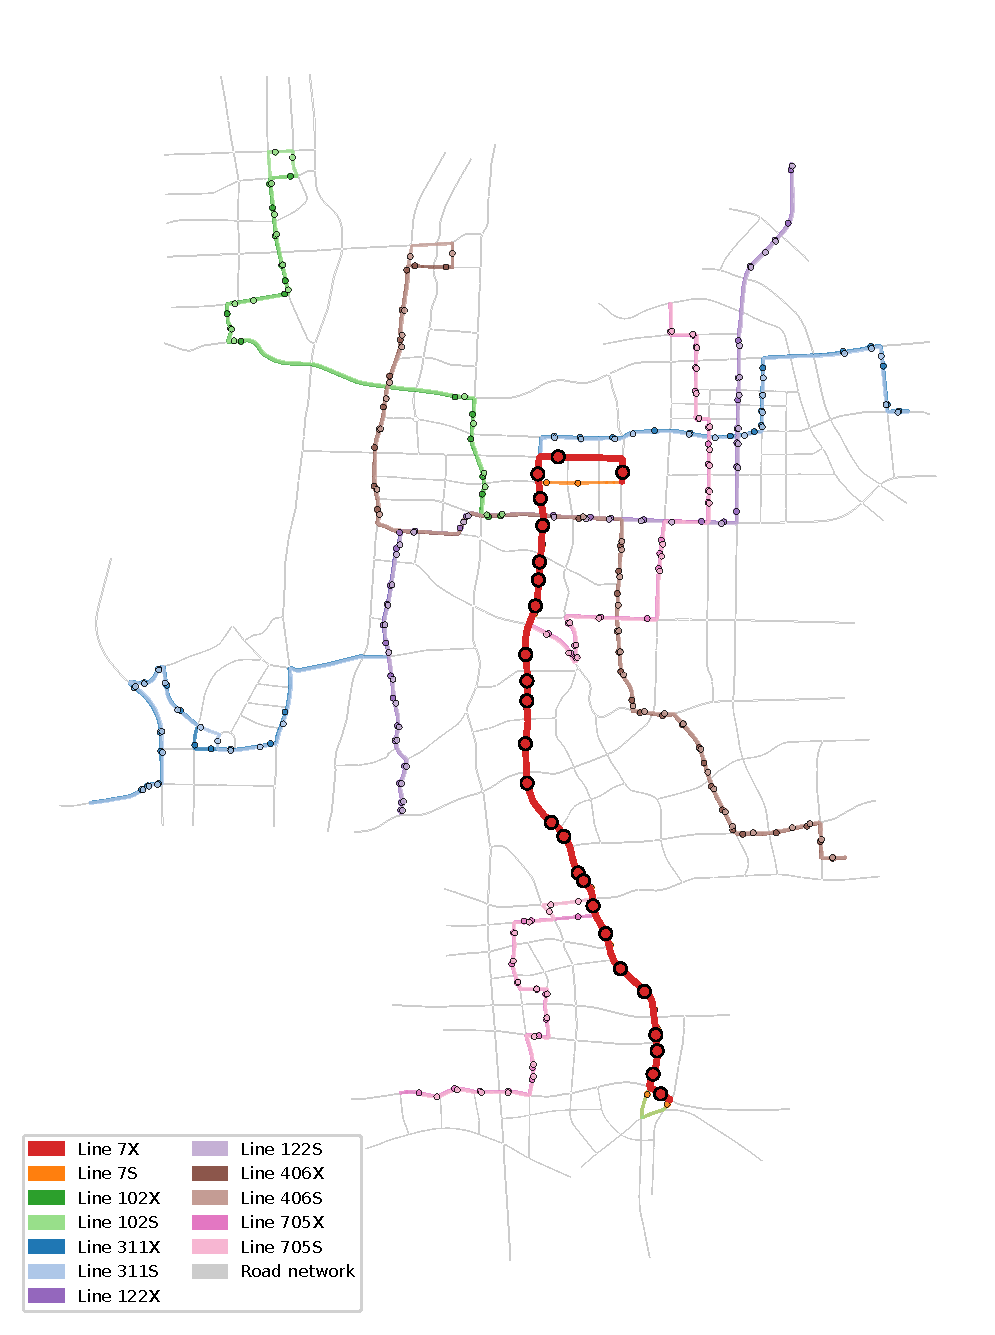
\includegraphics[width=0.70\linewidth]{figures/network_topology.pdf}
\caption{Topology of the twelve directional bus services represented in both
the target SUMO environment $\mathcal{M}_{\mathrm{tgt}}$ and the calibrated
online simulator $\mathcal{M}_{\mathrm{sim}}$. The two environments share stop
sequences, timetables, capacities, and passenger origin-destination journeys;
their traffic and event-propagation mechanisms differ. Line 7X is drawn more
heavily only for legibility; policy control covers all 12 services.}
\label{fig:network_topology}
\end{figure*}

\subsection{Offline-to-online learning objective}
\label{sec:problem:objective}

The immutable target replay is
\begin{equation}
\mathcal{D}_{\mathrm{off}}=
\left\{(s_{\iota},a_{\iota},r_{\iota},s'_{\iota},
\Gamma_{\iota},\Delta t_{\iota},z_{\iota})\right\}_{\iota=1}^{N_{\mathrm{off}}},
\qquad N_{\mathrm{off}}=3{,}284{,}718,
\label{eq:v7_dataset}
\end{equation}
In \Cref{eq:v7_dataset}, $\iota$ indexes an offline row,
$N_{\mathrm{off}}$ is the number of rows, and every tuple component follows
\Cref{eq:v7_state,eq:v7_action,eq:v7_discount,eq:v7_reward}. The data comprise
240 complete 24,000-s SUMO episodes: eight behavior policies crossed with 30
registered environment cells formed by ten independent seed blocks and three
demand scales. The behavior policies are zero holding, two random hurdle policies,
four schedule-adjusted headway-balance policies, and a closed-form myopic
welfare policy. They are used for coverage, not as claimed experts.

During learning, interaction is permitted only in
$\mathcal{M}_{\mathrm{sim}}$ and produces simulator replay
$\mathcal{D}_{\mathrm{sim}}$. No target-environment transition is queried
online. Given $\mathcal{D}_{\mathrm{off}}$ and a fixed simulator decision-event
budget, the H2O RL objective is
\begin{equation}
\max_{\pi}\;J_{\mathrm{tgt}}(\pi),
\qquad
J_{\mathrm{tgt}}(\pi)=
\E_{\mathcal{M}_{\mathrm{tgt}},\pi}
\left[\sum_{k=0}^{K-1}r_k\right],
\label{eq:v7_objective}
\end{equation}
where $J_{\mathrm{tgt}}(\pi)$ is the expected target-environment return,
$\E_{\mathcal{M}_{\mathrm{tgt}},\pi}$ takes expectation over the target kernel
and policy, $\pi$ is any admissible policy on the action space $[-1,1]$,
and $K$ is the number of
chronological decision tokens before the horizon. The objective in
\Cref{eq:v7_objective} is evaluated only after training. The learned policy is
$\pi_{\phi}$, with parameter vector $\phi$.
Within a fixed exogenous cell, \Cref{prop:ledger} implies that maximizing the
return and minimizing $Y$ give the same policy ordering. Across cells with
different passenger counts, unnormalized training returns and normalized
evaluation means need not assign the same relative weights to demand levels.
Importantly,
$R_{\mathrm{cmp}}$ in \Cref{eq:completion_rate} is not part of the training
reward; it is a separate service constraint at evaluation. This distinction
allows a policy to reduce accrued generalized passenger time while leaving more
journeys unfinished, and motivates the completion-aware transform in
\Cref{sec:method:reserve}. The setup otherwise matches the H2O setting
introduced by \citet{niu2022h2o} and studied by H2O+~\citep{niu2025h2oplus},
while keeping all evidence explicitly simulator-to-simulator.
